\documentclass{article}

\usepackage[utf8]{inputenc}
\usepackage[T1]{fontenc}
\usepackage{polski}
\usepackage{indentfirst}
\usepackage{lastpage}
\usepackage{natbib}
\usepackage{graphicx} 
\usepackage{sidecap}
\usepackage{wrapfig}
\usepackage{subfig}
\usepackage{caption}
\usepackage{geometry}
\usepackage{svg}
\usepackage{amsmath}

\usepackage{fancyhdr}
\pagestyle{fancy}
\fancyhf{}
\fancyheadoffset{0cm}
\rhead{P. Peszko}
\rfoot{Strona \thepage \hspace{1pt} z \pageref{LastPage}}
\lhead{Gra "Snake" sterowana sztuczną siecią neuronową.}
\title{Gra "Snake" sterowana sztuczną siecią neuronową. \\ Sprawozdanie końcowe}
\author{Patryk Peszko}
\date{4 czerwaca 2021}

\begin{document}
	\begin{titlepage}
		\clearpage\maketitle\thispagestyle{empty}
		\maketitle
	\end{titlepage}

\newpage
\newgeometry{tmargin=3cm, bmargin=3cm, lmargin=2cm, rmargin=2cm}
\thispagestyle{empty}
\tableofcontents
\newpage
\section{Wstęp}
    Ten dokument jest kontynuacja dokumentów pt. „Specyfikacja\_Funkcjonalna” oraz „Specyfikacja\_implementacyjna”. W tym dokumencie opiszę efekt końcowy projektu oraz jak on przebiegł.
\section{Cel Projektu}
    Celem projektu jest napisanie gry ”Snake” z graficznym interfejsem użytkownika (GUI), oraz zaimplementowanie sztucznej sieci neuronowej, która będzie sterować tą grą. Więcej o celu można przeczytać w dokumencie "Specyfikacja\_Funkcjonalna".
\section{Struktura projektu}
    Cały projekt zamieszczony jest w prywatnym repozytorium na stronie github.com.
    \subsection{Struktura plików}
        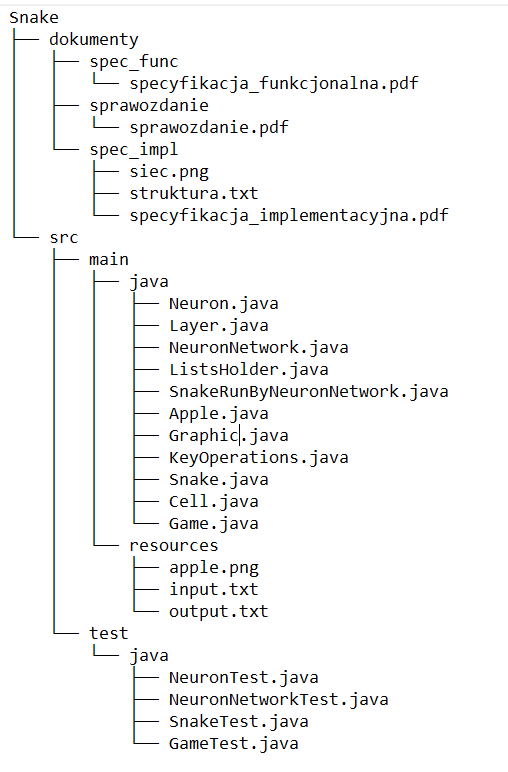
\includegraphics[scale = 2.2]{struktura}
\section{Różnice między efektem końcowym a celem opisanym w specyfikacjach.}
    \subsection{W funkcjonalności}
        \begin{itemize}
            \item Program nie umożliwia wczytanie pliku z współczynnikami sieci neuronowej.
            \item W GUI nie znajdziemy informacji na temat ilości pozostałych węży w następnej generacji. Zamiast tego widzimy średni wynik uzyskany przez węża od uruchomienia programu.
            \item Kliknięcie spacji powoduje rozpoczęcie gry. W trakcie trwania rozgrywki spacja umożliwia zatrzymanie i ponowne uruchomienie rozgrywki.
            \item Program nie zapisuje współczynników sieci neuronowej do pliku.
        \end{itemize}
    \subsection{W strukturze sieci neuronowej}
        \begin{itemize}
            \item Sieć składa się z 3 a nie z 4 warstw. Pierwsza warstwa liczy 13 neuronów a pozostałe po 3 neurony. Rozmiar sieci neuronowej został wybrany na podstawie analizy danych uzyskanych dla różnych rozmiarów sieci. Dane są dostępne w pliku "dane.xlsx".
            \item Neurony w pierwszej warstwie otrzymujące dane o lokalizacji jabłka mają stała wartość wynoszącą 1.
            \item Wszystkie neurony wykorzystują funkcje aktywacji sigmoidalną.
        \end{itemize}
        Sieć dostaje następujące informacje (zakładamy, że głowa jest zaznaczona na czerwono):
        \begin{itemize}
            \item 3 neurony wejściowe są odpowiedzialne za za sprawdzanie czy obok głowy nie znajduje się ściana. Jeżeli znajduje się to odpowiedni neuron otrzymuje 1 jako daną wejściową, przeciwnym wypadku 0.\\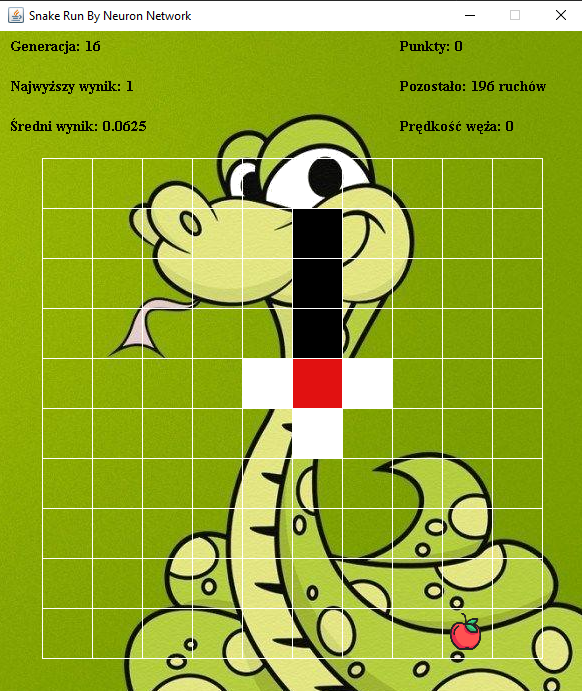
\includegraphics[scale = 1.9]{jablko}
            \item Sytuacja dla ogona jest analogiczna do powyższego przypadku.
            \item 7 neurony wejściowe są odpowiedzialne za za sprawdzanie czy w liniach prostych od głowy (zaznaczonych na poniższym zdjęciu) jest jabłko. Jeżeli znajduje się to odpowiedni neuron otrzymuje 1 jako daną wejściową, przeciwnym wypadku.\\ 
\includegraphics[scale = 2]{apple}
        \end{itemize}
    \subsection{W nienadzorowanym nauczaniu sieci}
        Zamiast algorytmu genetycznego zastosowałem propagację wsteczną błędu do uczenia sieci. Algorytm ten działa w następujący sposób. Głównym zadaniem sieci jest utrzymanie węża żywym. Jeżeli wąż "widzi" jabłko tzn. jeżeli jabłko leży na tej samej linii (bądź przekątnej) co głowa, to powinien skręcić w stronę jabłka o ile może. Jeżeli waż nie widzi jabłka to powinien iść dalej prosto (nie skręcać) o ile jest to możliwe. Jeżeli sieć podejmie decyzję niezgodną z tymi zasadami to zostaje zastosowany owy algorytm propagacji wstecznej błędu. Sieć uznaję za nauczoną gdy uzyska wynik powyżej 25. 
\newpage
\section{Testy}
    Napisałem testy dla wszystkich metod mogących zawierać potencjalnie błędy. Zdjęcie poniżej pokazuje, że wszystkie testy są zdawane i jakie metody zostały przetestowane.
    \\ 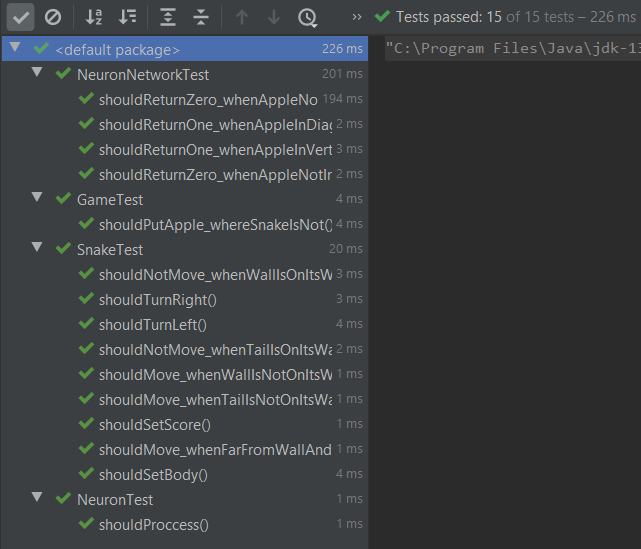
\includegraphics[scale = 2]{testy}
\section{Analiza danych uzyskanych dla różnych rozmiarów sieci.}
    Przetestowałem program dla sieci dla sieci o liczbie warstw ukrytych wynoszącej od 1 do 3 gdzie każda warstwa ukryta posiadała liczbę neurnów należacą do zbioru \{3,6,9\} neuronów. Dla każdego rozmiaru sieci testowałem również wartości stałe grup neuronów wejściowych. Podzieliłem je na 3 grupy:
    \begin{itemize}
        \item sprawdzające obecność ścian w pobliżu głowy
        \item sprawdzające czy ogon jest obok głowy
        \item sprawdzające czy jabłko jest w linii prostej od głowy
    \end{itemize}
    Wartości stałe należały do zbioru \{0,1,2,\}. Pełne dane są dostępne w pliku "dane.xlsx". Każda rozgrywka trwała 1000 generacji. Pod uwagę brałem zarówno liczbę uzyskanych punktów przez cała grę jak i najwyższy uzyskany wynik. Najwyższy wynik wyniósł 30 i uzyskały go 2 sieci. Pierwsza o jednej warstwie ukrytej posiadającej 3 neurony i o wartościach stałych odpowiednio dla grup wyżej wymienionych: 1, 0, 0. Druga sieć miała również jedną warstwę ukrytą ale zawierała ona 9 neuronów a stałe wartości miały odpowiednio: 2, 0, 1. \\
    Najwyższą średnia podczas całej rozgrywki uzyskała sieć o jednej warstwie ukrytej o 3 neuronach i wartościach stałych: 0, 2, 1.
    \\
    Wynik są odwrotnie proporcjonalne do rozmiarów sieci. Uważam to za ciekawy wynik ponieważ zakładałem, że będą potrzebne 2 warstwy ukryte po 18 neuronów.
\newpage
\section{Podsumowanie projektu}
    Projekt uznaję za sukces pomimo faktu, że wyniki nie zawsze są satysfakcjonujące. Najwyższy wynik (podczas zbierania danych 30, a generalnie 33) zdecydowanie przerósł moje oczekiwania co do tego programu. Niestety wyniki tak wysokie nie zdarzają się często. Najwyższy wynik powyżej 10 uzyskujemy mniej więcej co 2, 3 gry a powyżej 20 co 5, 6 gier. Jestem nieco zaskoczony, że jednak początkowy pomysł na wykorzystanie algorytmu genetycznego nie zadziałał. Jest również możliwe, że nie zadziałał ze względu na dużo większą sieć i inny algorytm sprawdzający gdzie powinna się udać sieć. \\
    Prace nad programem były prowadzone systematycznie ze względu na naglące terminy harmonogramu.\\
    Jestem bardzo zadowolony z nabytej wiedzy i świadomości, że potencjalnie tak proste rzeczy jak sieci neuronowe jednokierunkowe mogą zastąpić na po nauczeniu dużo bardziej skomplikowane algorytmy. Dzięki takiemu zabiegowi na pewno zaoszczędzimy na czasie uzyskując podobny wynik (a czasem taki sam). 
\end{document}
